\chapter{Resultados}

\begin{figure}[H]
  \centering
  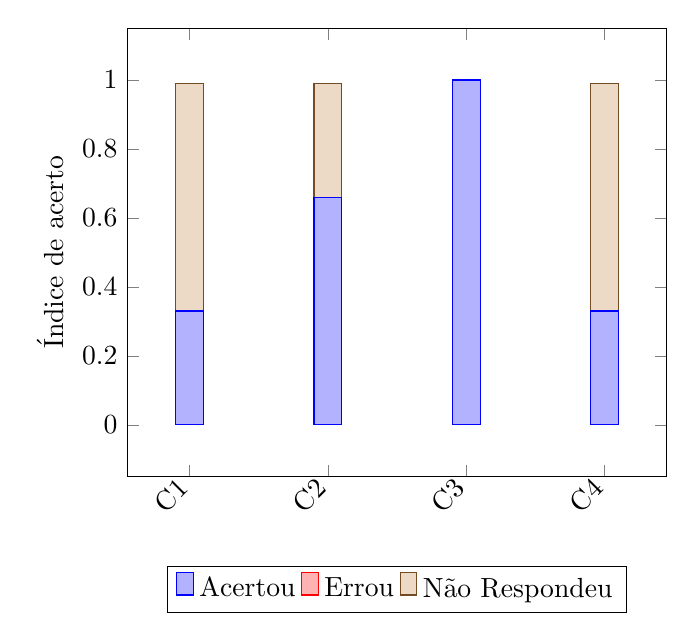
\begin{tikzpicture}
  \begin{axis}[
      ybar stacked,
      ymax=1,
      ymin=0,
      enlargelimits=0.15,
      legend style={at={(0.5,-0.20)},
        anchor=north,legend columns=-1},
      ylabel={Índice de acerto},
      symbolic x coords={C1, C2, C3, C4, 
          C5, C6, C7},
      xtick=data,
      x tick label style={rotate=45,anchor=east},
      ]
  \addplot+[ybar] plot coordinates {(C1,0.33) (C2,0.66) 
    (C3,1) (C4,0.33)};
  \addplot+[ybar] plot coordinates {(C1,0) (C2,0) 
    (C3,0) (C4,0)};
  \addplot+[ybar] plot coordinates {(C1,0.66) (C2,0.33) 
    (C3,0) (C4,0.66)};
  \legend{Acertou, Errou, Não Respondeu}
  \end{axis}
  \end{tikzpicture}
  \caption{Índice de acerto sem o uso da ferramenta}
\end{figure}

\begin{figure}[H]
  \centering
  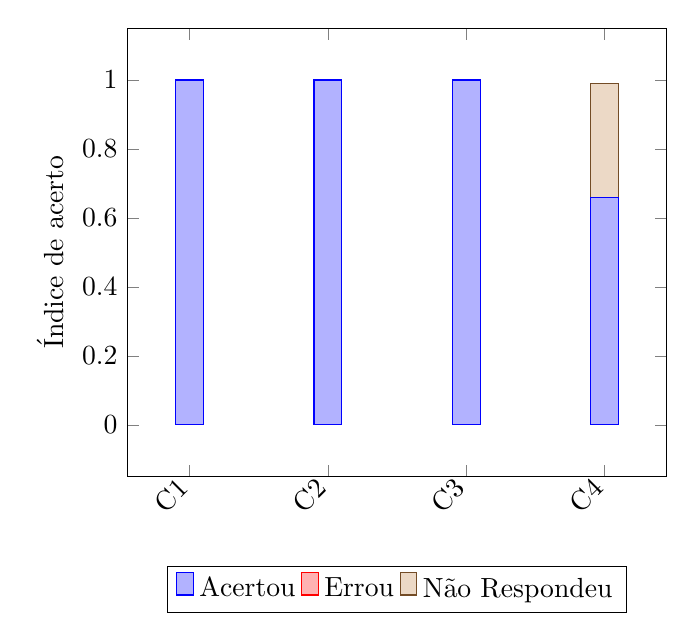
\begin{tikzpicture}
  \begin{axis}[
      ybar stacked,
      ymax=1,
      ymin=0,
      enlargelimits=0.15,
      legend style={at={(0.5,-0.20)},
        anchor=north,legend columns=-1},
      ylabel={Índice de acerto},
      symbolic x coords={C1, C2, C3, C4, 
          C5, C6, C7},
      xtick=data,
      x tick label style={rotate=45,anchor=east},
      ]
  \addplot+[ybar] plot coordinates {(C1,1) (C2,1) 
    (C3,1) (C4,0.66)};
  \addplot+[ybar] plot coordinates {(C1,0) (C2,0) 
    (C3,0) (C4,0)};
  \addplot+[ybar] plot coordinates {(C1,0) (C2,0) 
    (C3,0) (C4,0.33)};
  \legend{Acertou, Errou, Não Respondeu}
  \end{axis}
  \end{tikzpicture}
  \caption{Índice de acerto com o uso da ferramenta}
\end{figure}

\begin{figure}[H]
  \centering
  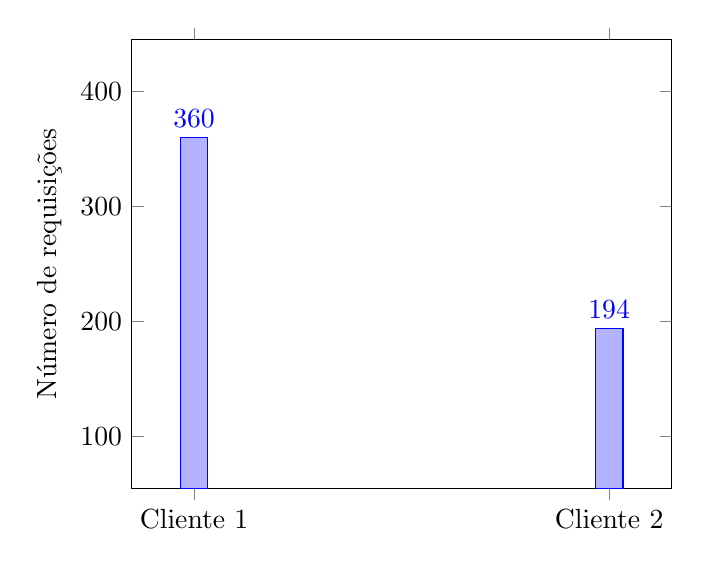
\begin{tikzpicture}
  \begin{axis}[
      ybar,
      ymax=400,
      ymin=100,
      enlargelimits=0.15,
      ylabel={Número de requisições},
      symbolic x coords={Cliente 1,Cliente 2},
      xtick=data,
      nodes near coords,
      nodes near coords align={vertical},
      ]
  \addplot coordinates {(Cliente 1,360) (Cliente 2,194)};
  \end{axis}
  \end{tikzpicture}
  \caption{Comparação no número de requisições C3}
\end{figure}

\begin{figure}[H]
  \centering
  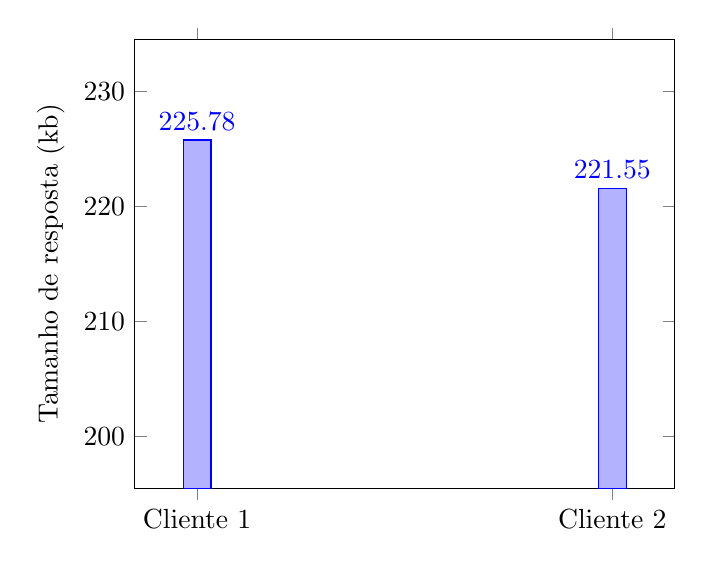
\begin{tikzpicture}
  \begin{axis}[
      ybar,
      ymax=230,
      ymin=200,
      enlargelimits=0.15,
      ylabel={Tamanho de resposta (kb)},
      symbolic x coords={Cliente 1,Cliente 2},
      xtick=data,
      nodes near coords,
      nodes near coords align={vertical},
      ]
  \addplot coordinates {(Cliente 1,225.777) (Cliente 2,221.547)};
  \end{axis}
  \end{tikzpicture}
  \caption{Comparação no tamanho de resposta C3}
\end{figure}

\begin{figure}[H]
  \centering
  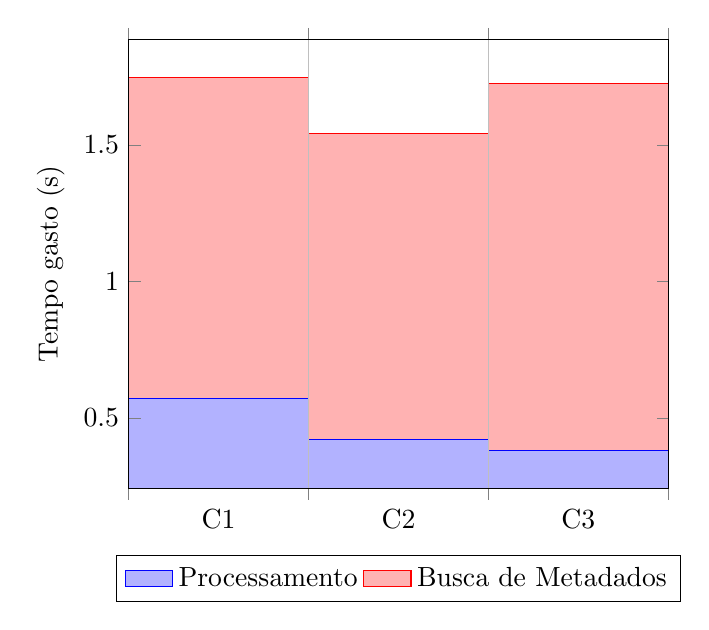
\begin{tikzpicture}
	\begin{axis}[
        ybar interval,
        ylabel={Tempo gasto (s)},
        legend style={at={(0.5,-0.15)},
        anchor=north,legend columns=-1},
        const plot,
		stack plots=y,
		area style,
        symbolic x coords={C1,C2,C3,C4},
		enlarge x limits=false]
	\addplot coordinates
		{(C1,0.57) (C2,0.42) (C3,0.38) (C4,0.48)}
		\closedcycle;
	\addplot coordinates
		{(C1,1.178) (C2,1.123) (C3,1.343) (C4,1.185)}
		\closedcycle;
    \legend{Processamento,Busca de Metadados}
	\end{axis}
  \end{tikzpicture}
  \caption{Overhead da ferramenta}
\end{figure}
